% Originally from a LyX file
\documentclass[english,conference,10pt]{IEEEtran}
\usepackage[T1]{fontenc}
\usepackage[utf8]{inputenc}
\usepackage{babel}
\usepackage{amsmath}
\usepackage{amsfonts}
\usepackage{amssymb}
\usepackage{units}
\usepackage{graphicx}
\usepackage{subcaption}
\usepackage[capitalise]{cleveref}
\crefname{equation}{}{}
\begin{document}

\title{Daala: Building A Next-Generation Video Codec From Unconventional
Technology}


\author{\author{\IEEEauthorblockN{Some authors\IEEEauthorrefmark{1}\IEEEauthorrefmark{2}}
\IEEEauthorblockA{\IEEEauthorrefmark{1}Mozilla Corporation, Mountain View, USA}\\
\IEEEauthorblockA{\IEEEauthorrefmark{2}Xiph.Org Foundation, USA}
}}
\maketitle
\begin{abstract}
Daala is a new royalty-free video codec based on perceptually-driven
coding techniques.
\end{abstract}


\section{Introduction}

Daala is a royalty-free video codec designed to avoid traditional
patent-encumbered techniques used in most current video codecs. One
of the goals of the Daala codec is to explore techniques that are
very different from those typically used in most codecs. Some of
these techniques are new to Daala, while others already existed, but
had not been applied to video coding before. While Daala is not yet
a competitive codec on its own, some of the techniques it uses are
currently being integrated in the Alliance For Open Media (AOM) AV1 codec.

\cref{sec:techniques} describes the non-traditional techniques used
in Daala and \cref{sec:AOM} discusses how these techniques fit within
the new AV1 codec. We then present some results obtained with Daala and AV1
in \cref{sec:Results}.

\section{Daala Techniques}
\label{sec:techniques}

One of the goals of the Daala codec is to explore techniques that
are very different from those typically used in most codecs. Most
of these techniques have been fundamental to Daala since the initial
stages of the project. In this description, a \textit{block} refers to
a square transform block, whereas a \textit{superblock} refers to the
largest area of a frame on which Daala can operate. Superblocks are $64\times 64$
pixels in Daala. Also, vector variables are denoted in bold, and quantized
variables are denoted with a hat.

\subsection{Lapped Transform}

Rather than using a deblocking filter to counter blocking artifacts, Daala uses a combination of pre- and post-processing filters at block edges to reduce or eliminate blocking artifacts~\cite{DaedeDCC}. Known as a Time-Domain Lapped Transform (TDLT)~\cite{MalvarS89,tran2003}, the set of filters used in Daala allow for perfect reconstruction for lossy or lossless operations at up to 12-bits per pixel~\cite{EggePCS}.

The post-processing filter is applied over block boundaries on the frequency domain coefficients. Therefore, the reconstructed bordering pixels are not available for intra-prediction, as they depend on the block currently being encoded. As a result, intra prediction is achieved in the frequency domain using either the first row of coefficients from the block above or the first column from the block to the left~\cite{EggePCS}.

\subsection{Haar DC}

Since Daala lacks intra prediction, the DCs of all transforms within a superblock
are transform-coded with a 2D Haar wavelet.
Also, DC coefficients are combined recursively using a Haar transform,
up to the level of the corresponding superblock. Since Daala transform blocks
are always split as quad-trees, the transform is applied bottom-up, recursively.
At each level, four DCs are combined into four Haar coefficients: one horizontal,
one vertical, one diagonal, and one new DC representing a larger block size.
The highest level ($64\times 64$) DC is predicted as a linear combination of the 
neighboring superblock DC coefficients: left, top-left, top, and top-right.

\begin{figure}
	\begin{minipage}[t]{0.49\columnwidth}
		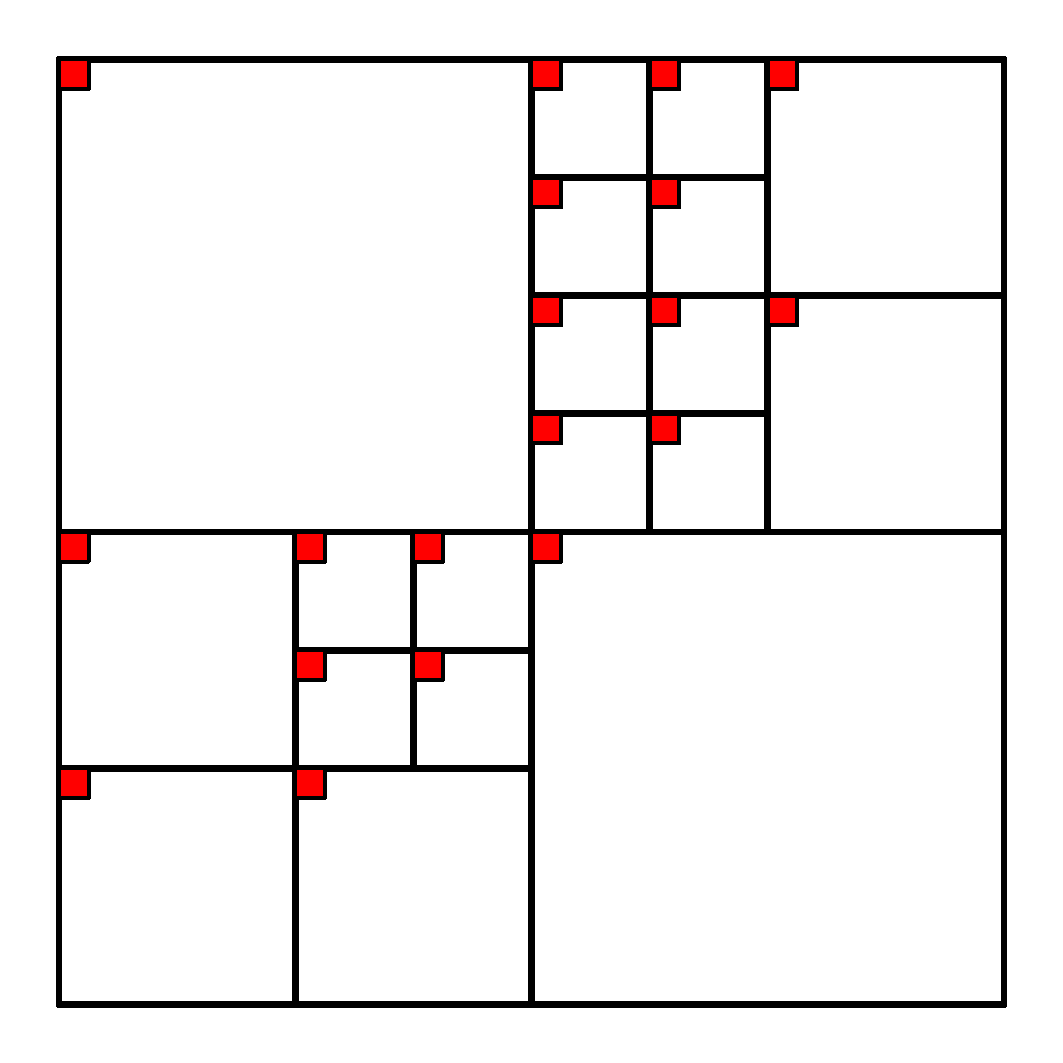
\includegraphics[width=\columnwidth]{block32_L0}
		\subcaption{Original DC coefficients before Haar DC}
	\end{minipage}
	\begin{minipage}[t]{0.49\columnwidth}
		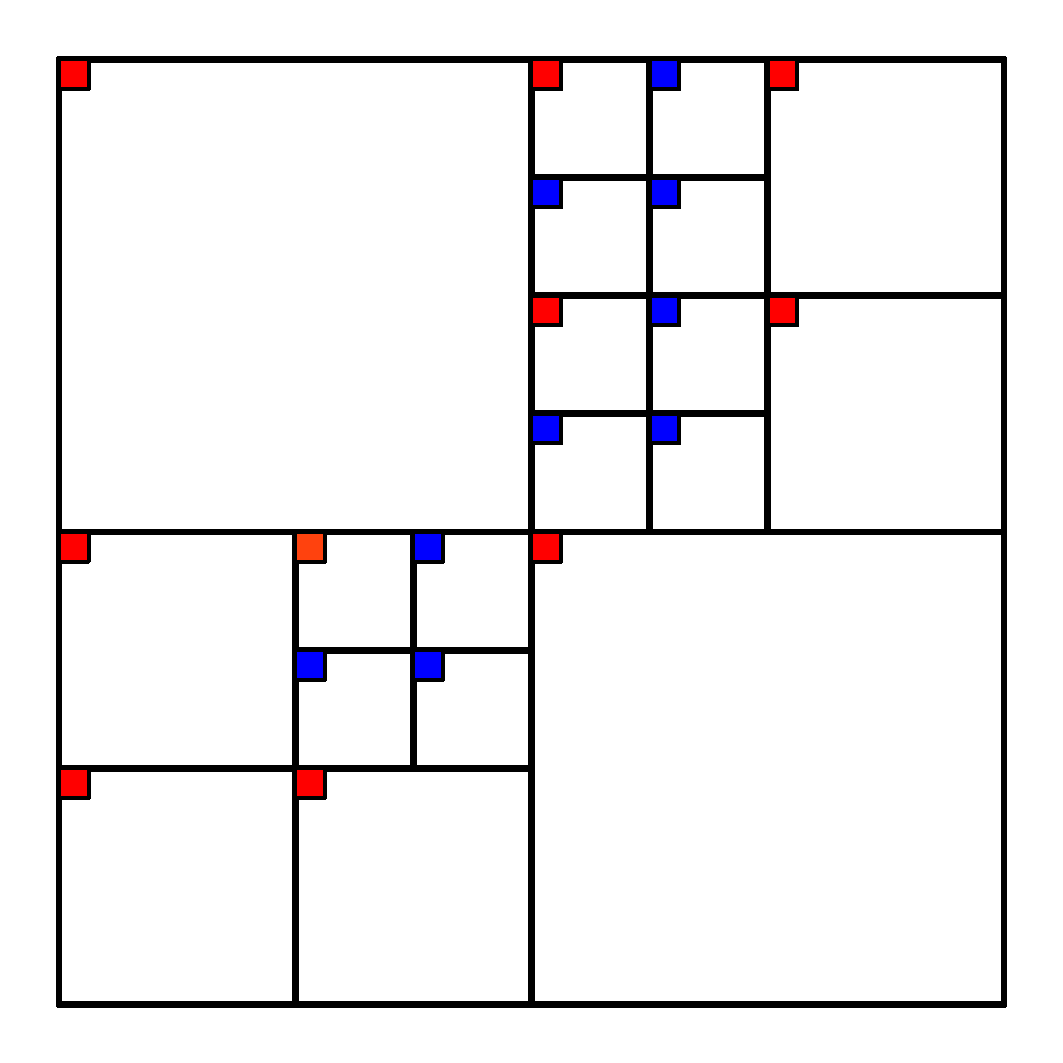
\includegraphics[width=\columnwidth]{block32_L1}
		\subcaption{DC coefficients from $4\times 4$ blocks are combined}
	\end{minipage}
	\begin{minipage}[t]{0.49\columnwidth}
		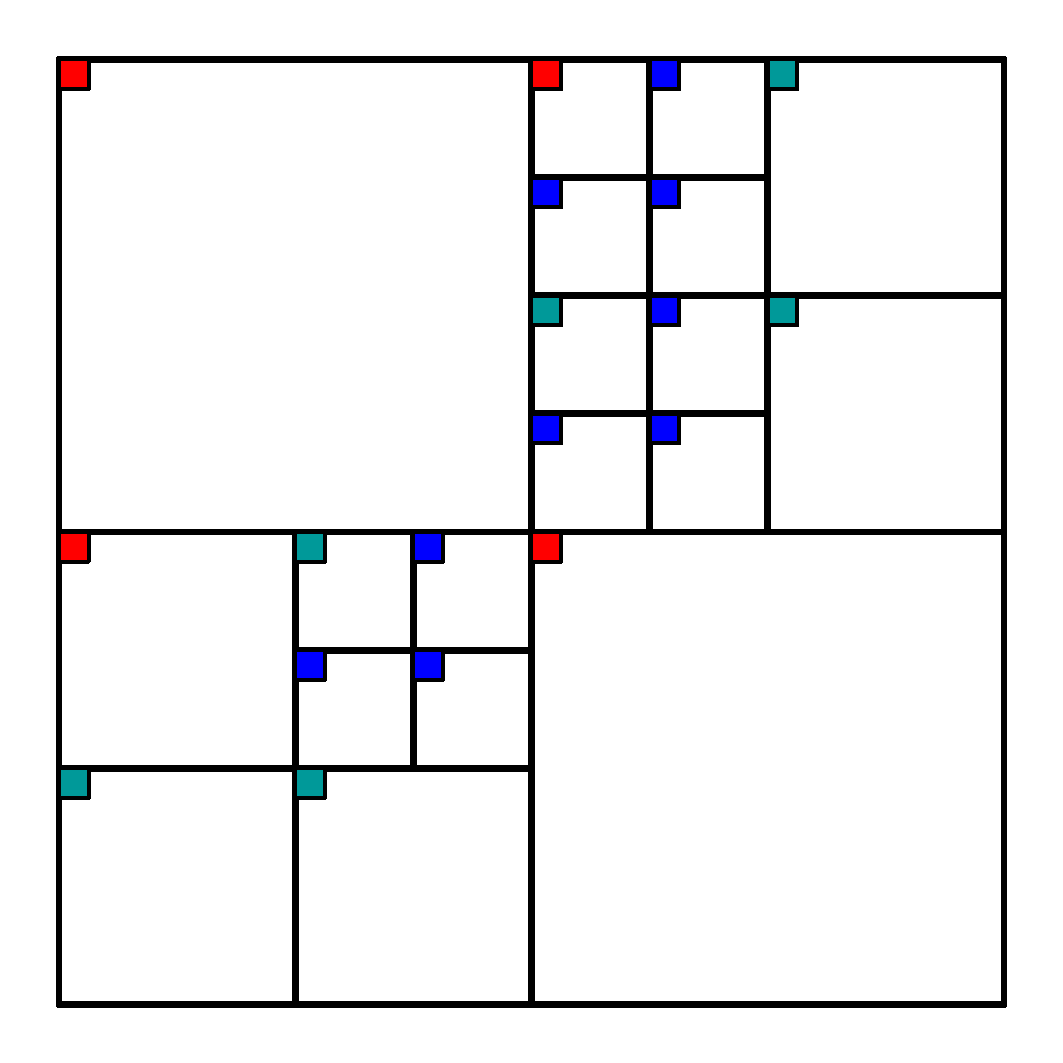
\includegraphics[width=\columnwidth]{block32_L2}
		\subcaption{DC coefficients from $8\times 8$ sub-blocks are combined}
	\end{minipage}
	\begin{minipage}[t]{0.49\columnwidth}
		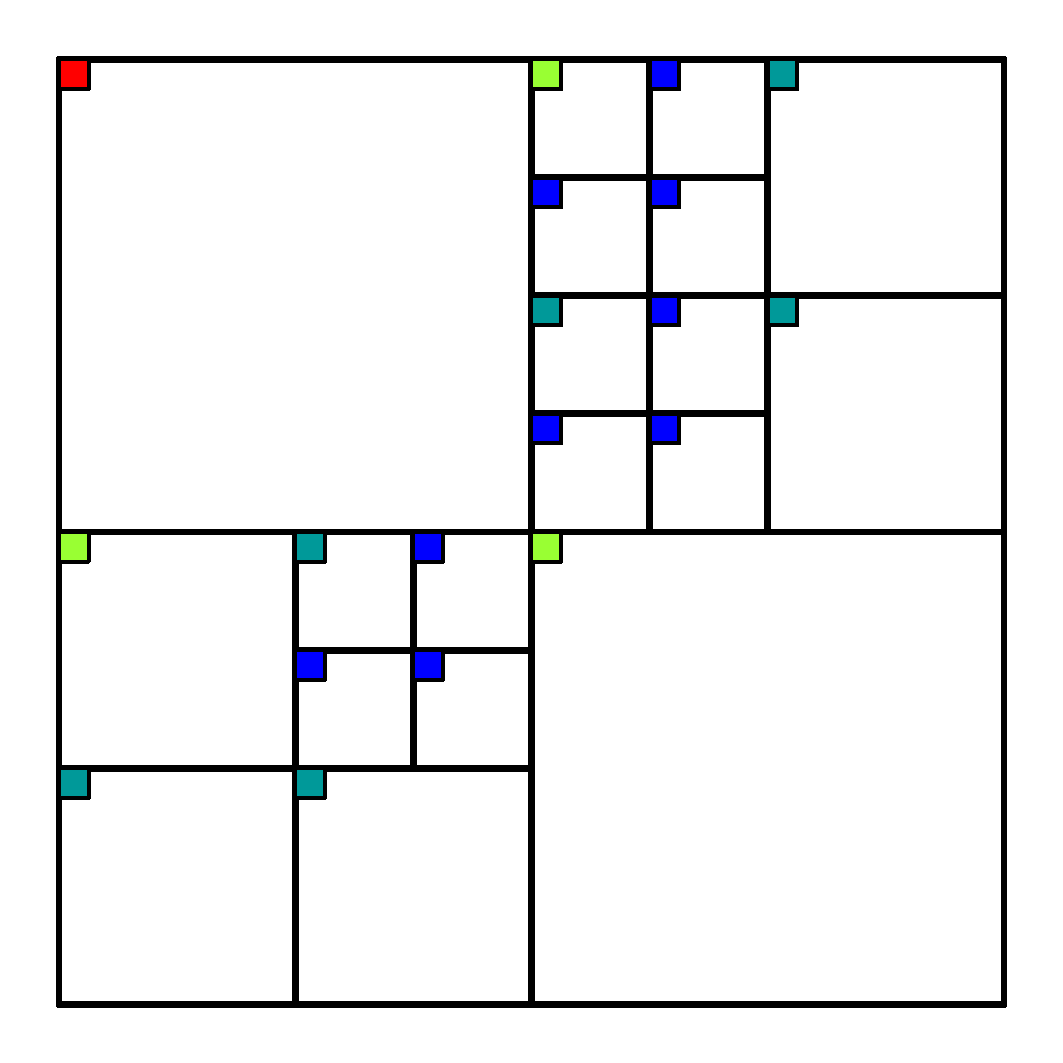
\includegraphics[width=\columnwidth]{block32_L3}
		\subcaption{DC coefficients from $16\times 16$ sub-blocks are combined}
	\end{minipage}
	\caption{Example of applying Haar DC over three levels on a $32\times 32$
		sub-block. The process is applied all the way to $64\times 64$. }
\end{figure}

\subsection{Multi-Symbol Entropy Coder}

Most recent video codecs encode information using binary arithmetic
coding, meaning that each symbol can only take two values. The Daala
range coder supports up to 16 values per symbol, making it possible
to encode fewer symbols~\cite{derfTools}. This is equivalent to
coding up to four binary values in parallel and reduces serial dependencies. 

To achieve this, Daala uses a multiply-free range coder approximation~\cite{stuiver1998piecewise}. 


\subsection{Overlapped Block Motion Compensation}

Because of the use of lapping we need a way to avoid blocking artifacts
in the prediction. For this we use overlapped block motion compensation
(OBMC)~\cite{OBMC}.


\subsection{Perceptual Vector Quantization}

In the majority of video codecs, motion-compensated reference frame
is subtracted from the input frame to compute a residual, which is
then transformed, and coded using scalar quantization. Daala differs
significantly from that description. Not only does it use vector quantization
rather than scalar quantization, but -- most importantly -- the motion-compensated
reference is never subtracted from the input frame. Instead, both
the motion-compensated reference is used to build a transformation
that makes the input easier to code. This technique is called perceptual
vector quantization (PVQ)~\cite{valin2015spie}.

Perceptual vector quantization originates in the pyramid vector quantizer
previously used for music in the Opus audio codec~\cite{ValinAES}. In Opus,
the pyramid vector quantizer is used as a gain-shape quantizer in a way that
ensures that the signal energy is always conserved. Using a gain-shape
quantizer in a video codec is more complicated, since we need to also take
into account a prediction. While it would be possible to quantize the difference
between the prediction and the input, conserving the energy of that
difference would be perceptually meaningless.

Rather than attempting to encode the difference, the prediction produces
a Householder reflection that makes the input easier to encode. Let 
$\mathbf{x}$ be the input and $\mathbf{r}$ be the prediction, we construct
 a Householder reflection plane
\begin{equation}
\mathbf{v} = \frac{\mathbf{r}}{\|\mathbf{r}\|} + s\mathbf{e}_m\ ,
\end{equation}
where $\mathbf{e}_m$ is a unit vector along dimension $m$ and $s = \pm1$.
The values of $m$ and $s$ can be chosen arbitrarily, but to maximize
numerical stability, we typically choose $m$ to be the position of the
largest absolute value in $\mathbf{r}$ and $s$ to be the sign of that value.

Once the reflection plane is computed, it is applied to the input vector
$\mathbf{x}$ to produce the reflected vector $\mathbf{z}$:
\begin{equation}
\mathbf{z} = \mathbf{x} - 2\frac{\mathbf{x}^T\mathbf{v}}
{\mathbf{v}^T\mathbf{v}}\mathbf{v}\ .
\end{equation}
When the input is similar to the prediction itself, the direction of the
reflected vector $\mathbf{z}$ is close $-\mathbf{e}_m$. To take advantage of
that fact, we express it as
\begin{equation}
\mathbf{z} = g\left(-s\cos\theta + \mathbf{u}\sin\theta\right)\ ,
\end{equation}
where $g$ is the magnitude of $\mathbf{z}$ (and thus also the magnitude of
$\mathbf{x}$), $\mathbf{u}$ is a unit vector with no component along the
$\mathbf{e}_m$ direction, and the angle $\theta$ representing the
similarity between the prediction and the input. Since the Householder
reflection is orthonormal, it follows that
\begin{equation}
\theta = \arccos\frac{\mathbf{x}^T\mathbf{r}}
                   {\left\|\mathbf{x}\right\|\left\|\mathbf{r}\right\|}\ .
\end{equation}

The unit vector $\mathbf{u}$ can be coded using a spherical quantizer derived
from the pyramid vector quantizer~\cite{Fischer1986}:
\begin{equation}
\mathbf{u}=\frac{\mathbf{y}}{\left\|\mathbf{y}\right\|}\ ,
\end{equation}
with
\begin{equation}
\mathbf{y} \in \mathbb{Z}^N : \left\|\mathbf{y}\right\|_{L1} = K \land y_m=0\ ,
\end{equation}
where the number of \textit{pulses} $K$ controls the size of the codebook.

The encoder quantizes $g$ and $\theta$ and encodes them in the bitstream along
with the integer vector $\mathbf{y}$ (except for $y_m=0$). The codebook
size $K$ is determined only from $g$ and $theta$ and does not need to be
transmitted. Since the decoder also has access to the prediction, the
reflection vector $\mathbf{v}$ and the values $m$ and $s$ do not need to
be transmitted. In total, there are $N-2$ degrees of freedom to code in
$\mathbf{y}$, with two more for $g$ and $\theta$, so the total is still
$N$ degrees of freedom. The main difference however is that two of the
coded values have a perceptual meaning: $g$ is the amount of contrast and
$\theta$ is the amount of change compared to the prediction. By coding $g$
as a parameter, it is easier to preserve the amount of contrast than by
coding only DCT coefficients.

In practice, the vectors $\mathbf{x}$ and $\mathbf{r}$ are transform
coefficients rather than pixel values. This requires an extra forward DCT
in both the encoder and the decoder since the input and the prediction need
to be transformed separately. Only the AC coefficients are coded using PVQ
and for blocks larger than $4\times 4$, the AC coefficients are divided into multiple
\textit{bands} where each band is coded separately. This makes it possible
to control the contrast separately, based on octave and direction.

PVQ makes it possible to take into account masking effects with no
extra signaling. Since the gain is explicitly signaled, it is easy to make
the quantization resolution dependent on the gain. This dependency can be
expressed as
\begin{equation}
E\left\lbrace \left\| \mathbf{x} - \hat{\mathbf{x}} \right\|^2 \right\rbrace
\propto g^{2\alpha}\ , 0 \leq \alpha \leq 1\ ,
\end{equation}
where $\alpha=0$ behaves like a standard linear scalar quantizer and
$\alpha=1$ produces a constant relative error like in the Opus audio codec.
Daala uses $\alpha = \nicefrac{1}{3}$. To achieve this, we quantize the
companded gain
\begin{equation}
\gamma = g^{1-\alpha}\ ,
\end{equation}
giving finer resolution to smaller gains and coarser resolution to larger
gains.

The decoder always decodes the quantized companded gain $\hat{\gamma}$
first. From there it can compute the quantization step size for $\theta$ as
\begin{equation}
Q_\theta = \frac{\beta}{\hat{\gamma}}\ ,
\end{equation}
where $\beta = 1/(1-\alpha)$.

The size of the codebook $K$ was determined through curve
fitting~\cite{valin2015spie} to be
\begin{equation}
K = \frac{\hat{\gamma}\sin\hat{\theta}}{\beta}\sqrt{\frac{N+2}{2}}\ .
\label{eq:K_nonrobust}
\end{equation}
The formulation in~\cref{eq:K_nonrobust} is not robust to packet loss when
the gain is predicted (leading the decoder to obtain the wrong $K$ and decode
the wrong number of symbols). Fortunately, by making the $\sin{\hat{\theta}}
\simeq \hat{\theta}$ approximation and substituting $\hat{\theta} = 
Q_\theta\hat{\tau}$, where $\tau$ is the angle quantization index, we obtain
\begin{equation}
K = \tau \sqrt{\frac{N+2}{2}}\ .
\end{equation}


\subsection{Chroma from Luma (CfL) Prediction}

Although the use of $\mathrm{Y'C_BC_R}$ reduces the correlation across planes
compared to RGB, there still exists a correlation between the chroma planes
$\mathrm{C_B}$ and $\mathrm{C_R}$ and the luma plane Y'. Edges in chroma tend to
align very well with edges in luma with only the amount of contrast (gain) differing.
Because of that property, PVQ makes it especially easy to predict
chroma planes from the luma plane. Daala's chroma from luma (CfL)~\cite{egge2015spie}
prediction directly uses the luma transform coefficients as the prediction vector
$\mathbf{r}$ for coding the chroma coefficients with PVQ. The main difference compared
to the normal way of using PVQ is that a sign needs to be coded for the prediction
(since the luma plane and chroma plane coefficients may be negatively correlated) and
that the gain of the chroma cannot be predicted from the gain of the luma.


\subsection{Directional Deringing Filter}
\label{sec:deringing}

Like other transform codecs, Daala can cause ringing artifacts around edges.
The directional deringing filter attempts to eliminate the ringing without
blurring the image. Unlike the HEVC Sample-Adaptive Offset (SAO)~\cite{HEVC-SAO},
the Daala deringing filter is not based on classifying pixels and applying per-class
offsets. Instead, it is a directional outlier-robust filter that smooths the
neighborhood of pixels while preserving edges.

Let $x\left(n\right)$ denote a 1-dimensional signal and $w_{k}$
denote filter tap weights, a linear finite impulse response (FIR)
filter with unit DC response is defined as
\begin{equation}
y\left(n\right)=\frac{1}{\sum_{k}w_{k}}\sum_{k}w_{k}x\left(n+k\right)\ ,\label{eq:FIR1}
\end{equation}
which can alternatively be written as
\begin{equation}
y\left(n\right)=x\left(n\right)+\frac{1}{\sum_{k}w_{k}}\sum_{k,k\neq0}w_{k}\left[x\left(n+k\right)-x\left(n\right)\right]\ .\label{eq:FIR2}
\end{equation}
The main advantage of expressing a filter in the form of~\cref{eq:FIR2}
is that the normalization term $\frac{1}{\sum_{k}w_{k}}$ can be approximated
relatively coarsely without affecting the unit gain for DC. This makes
it easy to use small integers for the weights $w_{k}$.

The disadvantage of linear filters for removing ringing artifacts
is that they tend to also cause blurring. To reduce the amount of
blurring, the conditional replacement filter used in Daala excludes
the signal taps $x\left(n+k\right)$ that would cause blurring and
replaces them with $x\left(n\right)$ instead. This is determined
by whether $x\left(n+k\right)$ differs from $x\left(n\right)$ by
more than a threshold $T$. The FIR filter in~\cref{eq:FIR2}
then becomes a conditional replacement filter expressed as
\begin{equation}
y\left(n\right)=x\left(n\right)+\frac{1}{\sum_{k}w_{k}}\sum_{k,k\neq0}w_{k}R\left(x\left(n+k\right)-x\left(n\right),T\right)\ ,\label{eq:CRF}
\end{equation}
where
\begin{equation}
R\left(x,T\right)=\left\{ \begin{array}{ll}
x & ,\ \left|x\right|<T\\
0 & ,\ \mathrm{otherwise}
\end{array}\right.\ .
\end{equation}

To further reduce the risk of blurring the decoded image, the conditional
replacement filter is applied along the main direction of the edges
in each $8\times 8$ block. The direction is determined based on the decoded image
(no side information transmitted) by analyzing each $8\times 8$ block as described
in~\cite{ValinDeringing}. For each $8\times 8$ block, the decoder determines which
of eight different directions best represents the content of the block.
The search can be efficiently implemented in SIMD. To filter a pixel, a 7-tap
conditional replacement filter is applied along the detected direction.
The process is repeated for each pixel in each block being filtered.

To further reduce ringing in very smooth regions of the image, the filter
is applied a second time to combine multiple output values of the
first filter. The second filter is applied either vertically or horizontally
-- in the direction most orthogonal to the one used in the first filter.
For example, for a 45-degree direction, the second filter would be
applied horizontally. The combined effect of the two filters is a separable
deringing filter that covers a total of 35~pixel taps.


\section{Alliance for Open Media AV1 codec}
\label{sec:AOM}

Some of the techniques used in Daala are currently being considered for
inclusion in the Alliance for Open Media (AOM) AV1 video codec. The
deringing filter described in \cref{sec:deringing} is already
fully integrated in AV1 and has been shown to reduce bitrate by around 2\%
at equal quality. 

The multi-symbol entropy coder is also being evaluated. Using the piecewise
integer mapping exactly as described in~\cite{stuiver1998piecewise} results
in a bitrate overhead of around 1\%. However, we have experimented with
better approximations that do not have such cost and assume that
the denominator of the probabilities is a power of two.

PVQ is early stages of experiments in AV1 and is by far the most invasive
of the techniques under consideration, as it requires changes in some
of the signaling, as well as the addition of a forward transform on the
prediction itself. No results are available yet, but should PVQ be
included in AV1, it would make it possible to also experiment with CfL.

Lapped transforms and OBMC are \textit{not} being considered for inclusion
in AV1. Both these techniques have far-reaching interactions with the
other coding techniques and would essentially require a complete re-design
of the codec. 

\section{Results}
\label{sec:Results}


\section{Conclusion}

\bibliographystyle{IEEEtran}
\bibliography{daala}

\end{document}
